%%% Version 4.4 Generated 2018/06/15 %%%
\documentclass[utf8]{style/FrontiersinHarvard}
\usepackage{url, hyperref, lineno, microtype}
\usepackage[onehalfspacing]{setspace}

\usepackage{multirow}
\usepackage{xspace}
\usepackage{siunitx}
\usepackage[version=4]{mhchem}
\usepackage{textcomp} % registered trademark and copyright symbols
\usepackage{graphicx, subcaption}

% See mode, number-mode and unit-mode; values are text, math, and match
\sisetup{separate-uncertainty=true, 
    exponent-product=\cdot,
    per-mode=symbol,
    mode = text,
    range-units=single}
\DeclareSIUnit{\year}{yr}
\graphicspath{{"figures/"}}

% \linenumbers
\def\keyFont{\fontsize{8}{11}\helveticabold }

% Set author information
% --------------------------------------------- %
\def\firstAuthorLast{Sample {et~al.}}
\def\Authors{Mastnak, Elijan J.\,$^{1,*}$, Djordević, Srdjan\,$^{2}$ and Krašna, Simon\,$^{3}$}
\def\Address{$^{1}$University of Ljubljana, Faculty of Mathematics and Physics, Ljubljana, Slovenia. elijan-jakob.mastnak@student.fmf.uni-lj.si \\
$^{2}$TMG-BMC Ltd., Štihova ulica 24, 1000 Ljubljana, Slovenia. srdjand@tmg.si \\
$^{3}$University of Ljubljana, Faculty of Mechanical Engineering, Ljubljana, Slovenia. simon.krasna@fs.uni-lj.si}
\def\corrAuthor{Elijan Mastnak}
\def\corrEmail{elijan-jakob.mastnak@student.fmf.uni-lj.si}
% --------------------------------------------- %

% Define custom macros
% --------------------------------------------- %
\newcommand{\TODO}[1]{{\textbf{TODO:} {\color{red} #1}}}

% TMG parameters
% --------------------------------------------- %
\newcommand{\Dm}{\ensuremath{\text{Dm}}\xspace}
\newcommand{\Td}{\ensuremath{\text{Td}}\xspace}
\newcommand{\Tc}{\ensuremath{\text{Tc}}\xspace}
\newcommand{\RDDMax}{\ensuremath{ \text{RDD}_{\text{max}}}\xspace}
\newcommand{\RDDMaxTime}{\ensuremath{ \text{TRDD}_{\text{max}}}\xspace}
% --------------------------------------------- %

% SPM parameters
% --------------------------------------------- %
\newcommand{\SPMStart}{\ensuremath{\text{SPMStartTime}}\xspace}
\newcommand{\SPMEnd}{\ensuremath{\text{SPMEndTime}}\xspace}
\newcommand{\SPMCentroidTime}{\ensuremath{\text{SPMCentroidTime}}\xspace}
\newcommand{\SPMCentroidT}{\ensuremath{\text{SPMCentroid}}\xspace}
\newcommand{\SPMMax}{\ensuremath{\text{SPMMax}}\xspace}
\newcommand{\SPMArea}{\ensuremath{\text{SPMArea}}\xspace}
% --------------------------------------------- %

\begin{document}
\onecolumn
\firstpage{1}

\title[Quantifying Twitch Potentiation with TMG and SPM]{Quantifying Post-Activation Twitch Potentiation with Tensiomyography and Statistical Parametric Mapping} 

\author[\firstAuthorLast ]{\Authors}
\address{}
\correspondance{}
\extraAuth{}

\maketitle

% The abstract should render the general significance and conceptual advance of the work clearly accessible to a broad readership.
\begin{abstract}
\section{}
This study proposes and demonstrates in practice the use of statistical parametric mapping for reliably detecting and quantifying post-activation twitch potentiation in superficial skeletal muscles.
The study applies SPM to tensiomyographic measurements of the rectus femoris muscle's contractile response during electrically-induced twitch contraction following a conditioning exercise. SPM was found to reliably and quantitatively differentiate between the muscle's pre-conditioning and post-conditioning response, indicating the presence of post-activation potentiation.
More so, because SPM preserves the time-domain information contained in the original muscle response, SPM shows exactly \textit{when} the potentiation-like state occurred over the course of the muscle twitch.

\tiny
\keyFont{\section{Keywords:} tensiomyography, statistical parametric mapping, twitch potentiation, post-activation potentiation, neuromuscular electrical stimulation}
% Provide 5-8 keywords
\end{abstract}

\section{Introduction}
In the phenomenon generally called post-activation potentiation, a short, intense burst of muscle activity (called a \textit{conditioning exercise} in this context) temporarily increases the amplitude, force, and speed of both voluntary and electrically induced muscle contractions that immediately follow.
[14][15][1][16][17].

In general, prior muscle activity produces two different---and potentially coexistent---muscle responses: fatigue and potentiation.
Limited by the inevitable onset of fatigue, one cannot use conditioning exercises to increase subsequent muscle performance via potentiation ad infinitum---eventually fatigue outweighs any potentiation-like performance improvement.
Fatigue can coexist with PAP [18], and measured muscular performance represents the net balance between processes that cause fatigue and processes that cause potentiation [18].
Striking a favorable balance between fatigue and potentiation should be of interest to coaches, sports scientists, and athletes alike.
Doing so requires a reliable means of detecting and quantifying potentiation, and this article offers a novel way of doing so---directly in the time domain in which the muscle response is originally measured.

\subsection{On PAP, PAPE, and twitch potentiation}
We pause briefly to comment on some ambiguity in the literature surrounding post-conditioning enhancements in muscular performance,
generally involving confusion between the following two phenomena.
% \cite{prieske}
\begin{itemize}

    \item \textit{Post-activation potentiation} (PAP) is a short-term enhancement in a muscle's contractile properties during an electrically-induced muscle twitch, which generally manifests as enhanced twitch force and amplitude, and decreased time to peak contraction.
    PAP has a short half-life ($ \sim \SI{30}{\second} $),
    % \cite{vandervoort}
    is verified at the specific level of an individual muscle using a non-voluntary, electrically-induced muscle twitch, and generally requires nontrivial equipment and a standardized test environment to measure.
% study in a controlled, systematic manner.

    \item \textit{Post-activation performance enhancement} (PAPE) is
    a somewhat longer-term performance improvement in exercises serving as measures of maximal strength, power, and speed (e.g. a maximum vertical jump or a 60-meter sprint).
    PAPE has a longer half-life (maximum performance enhancement occurs on the order of 5 to 10 minutes following the initial conditioning exercise),
    % \cite{wilson}
    is verified at a macroscopic level by observing exercise performance (rather than measuring the contractile properties of a specific muscle),
    and is thus simpler to measure than than PAP, possibly at the expense of a less controlled and systematic experiment.

\end{itemize}

The present study concerns PAP, i.e. the short-term, post-conditioning enhancement in muscular contractile properties during electrically-induced twitch, and for this reason we will tend to use the more specific term \textit{twitch potentiation}.
Borrowing the definition of Hodgson et al (2005) [2],
``a twitch is a brief muscle contraction in response to a single presynaptic action potential or a single, synchronised volley of action potentials.''
Twitch potentiation (TP) is a well-established and reproducible phenomenon that manifests as both enhanced muscle twitch amplitude [19][27][28] and decreased time to attaining maximum amplitude [4] \cite{sale} [21].

TP has been demonstrated using electrically induced twitch contractions and attributed to phosphorylation of myosin regulatory light chains [21], which makes actin and myosin more sensitive to \ce{Ca^2+} ions [2]
The muscle's potentiated state has also been attributed to an increase in $ \alpha $-motoneuron excitability [16].
Fatigue induces a decrease in amplitude and velocity of twitch contraction, while PAP causes an increase in amplitude and velocity of twitch contraction and thus enhanced contractile response [4][2][3].

\subsection{Quantifying potentiation}
Currently, it is standard to quantify the level of twitch potentiation using discrete twitch contraction parameters computed retrospectively from measurements of muscle displacement, force production, or electrical activity with respect to time.
Examples of these parameters include maximal amplitude of muscle contraction, time taken to reach peak contraction, maximal twitch rate of force development [29][30][31], and peak M-wave amplitude [3].
In each case, computing these parameters reduces the originally-measured muscle response, which is generally a one-dimensional time series (e.g. muscle displacement with respect to time), to a single number, i.e. a zero-dimensional scalar value.
Based on the values of these parameters, one then retrospectively infers if the muscle response from which they were computed corresponded to a potentiated state.

A promising new approach to quantifying TP would analyze 
muscle response and detect and quantify potentiation directly in the time domain in which the muscle response was originally measured, without the dimensionality reduction imposed by computing discrete twitch contraction parameters.
One way of performing such an analysis is the method of statistical parametric mapping (SPM) [32][33][34][35].

Borrowing the definition of Flandin and Friston \cite{flandin}, 
``Statistical parametric mapping is the application of random field theory to make inferences about the topological features of statistical processes that are continuous functions of space or time''.
SPM has so far found its greatest application in neuroimaging for detecting regionally-specific brain activations \cite{friston}.
We use SPM similarly in the present study---applied to one-dimensional functions of time (i.e. twitch amplitude with respect to time) instead of three-dimensional functions of space (i.e. brain scans)---to detect regionally-specific variations between pre-conditioning and post-conditioning muscle responses directly in the time domain.
Statistically significant variations between pre-conditioning and post-conditioning muscle responses are then interpreted as post-activation potentiation.
Most promisingly, because SPM preserves the time-domain information contained in the original muscle response, SPM gives an indication of \textit{when} the potentiation-like state occurred over the course of the muscle twitch.
Of course SPM and conventional twitch contraction parameters are far from mutually exclusive as a means of detecting and quantifying potentiation---in fact the two may be used simultaneously, as the present study illustrates.

Quantifying twitch potentiation, then, requires two things: a means of measuring a muscle's contractile response following a conditioning exercise and a technique for analyzing the measured muscle response that can determine the presence (or lack) of potentiation.
Tensiomyography (TMG) is a standard method for selectively measuring contractile response and assessing twitch contraction parameters in superficial skeletal muscles [36][37][38][39][40][41][42].
This study assessed TP in a sports training setting by analyzing TMG measurements of electrically-induced muscle contraction both
\begin{enumerate}

    \item using SPM applied directly to TMG muscle responses in the time domain, and

    \item using discrete (zero-dimensional) TP parameters, computed retrospectively from the measured TMG signal, that summarize the muscle's twitch contraction properties.

\end{enumerate}
The study aimed to find if TMG measurement of muscle response followed by SPM analysis of this response can accurately and consistently identify statistically significant differences in the pre- and post-conditioning contractile response of the rectus femoris muscle, and,
if yes, to identify and quantify the associated time-domain changes of twitch potentiation.

\section{Materials and Methods}
\subsection{Participants}
The present study analyzed 55 subjects (age \SI{28.17 \pm 10.9}{\year}; height \SI{178.15 \pm 10.43}{\centi \meter}; weight \SI{71.84 \pm 12.82}{\kilogram}; 28 male and 27 female; 38 elite athletes and 17 recreational).
% TODO describe the simple random random sampling strategy?
To be approved for participation, subjects were required to be injury-free at the beginning of the testing protocol.
The intention and experimental procedure was described to all subjects, and written informed consent was obtained.
The investigation was approved by the Institutional Research Ethics Committee (University of Belgrade, Faculty of Sport and Physical Education), following the recommendations of the Declaration of Helsinki.

\subsection{Study Design}

\subsubsection{Tensiomyography specifications}
The study used tensiomyograhy (TMG) to measure the pre-conditioning and post-conditioning contractile responses of the rectus femoris (RF) muscle.
TMG measurements were taken with the TMG S1 measurement system (TMG-BMC, Ljubljana, Slovenia), which uses an opto-inductive sensor with a spring of spring constant \SI{0.17}{\newton \per \milli \meter} that generates an initial pressure of approximately \SI{1.5e-2}{\newton \per \milli \meter \squared} on a tip area of \SI{11.34}{\milli \meter \squared}.
Two self-adhesive electrodes (UltraStim\textregistered{} Wire, Axelgaard, USA) were positioned approximately along the anatomical axis of the femur, proximal on the beginning of RF and distal \SI{10}{\centi \meter} apart [11], symmetrically \SI{2}{\centi \meter} from the sensor on the RF muscle.
The positive electrode (anode) was placed proximally, and the negative electrode (cathode) distally, as shown in Figure~~\ref{fig:electrodes}.
% TODO: image of sensor position

\begin{figure}[htb!]
	\centering
    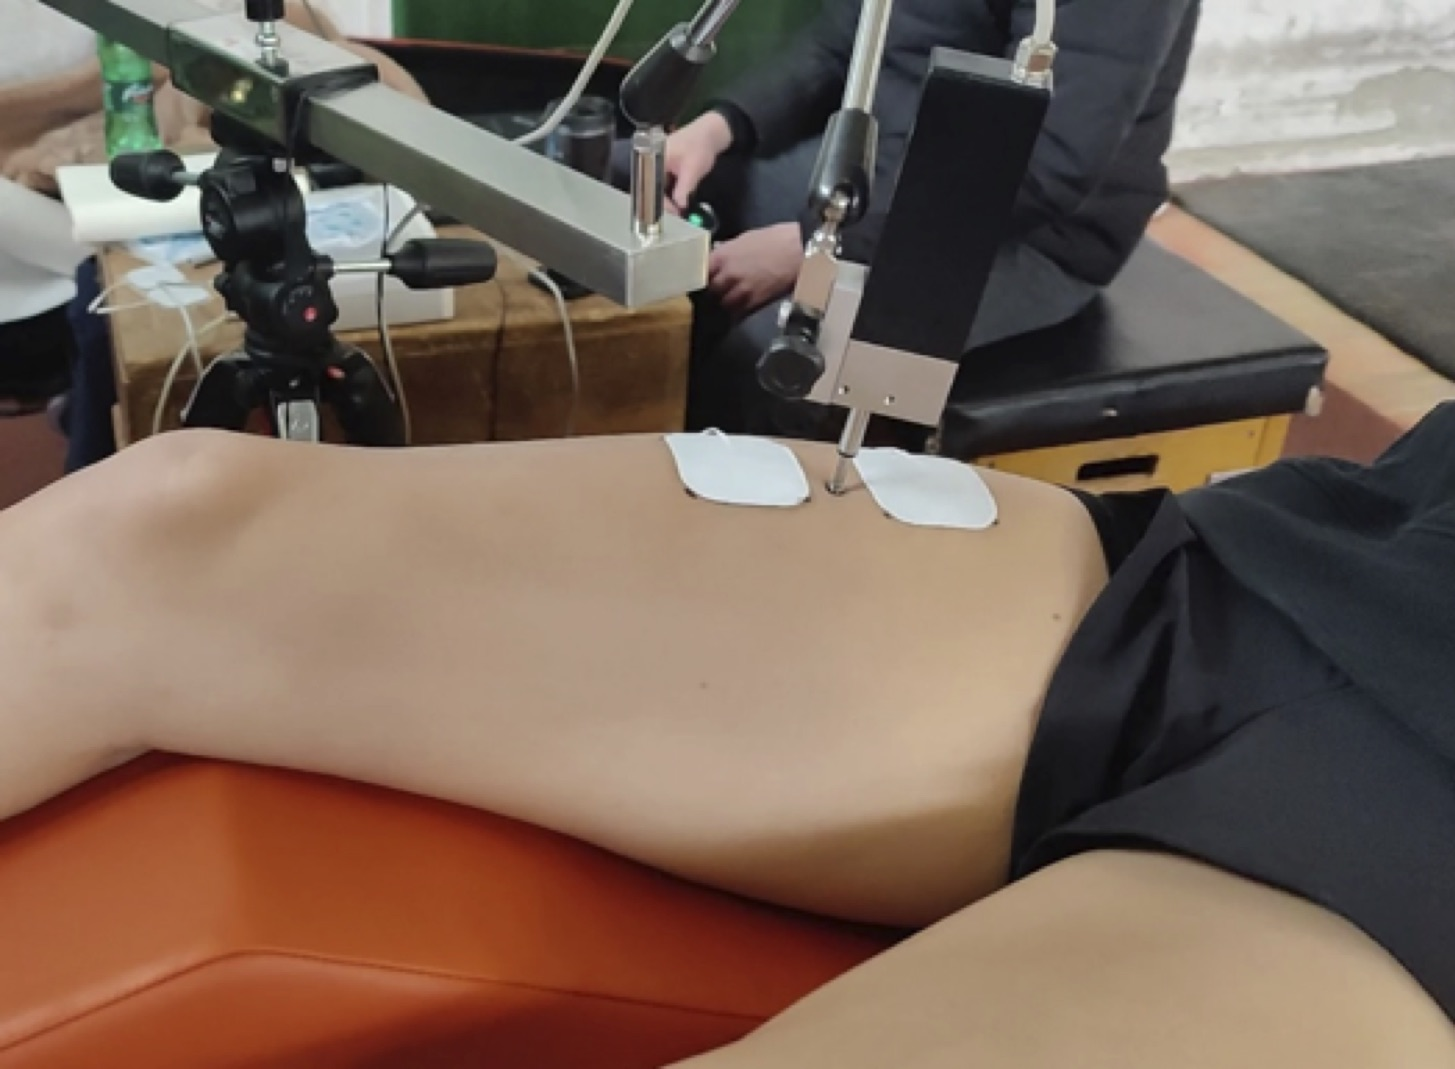
\includegraphics[width=0.65\textwidth]{word/electrodes.jpg}
    \caption{The position of the electrodes used for muscle simulation.}
    \label{fig:electrodes}
\end{figure}

The electrodes remained fixed on the skin for the duration of the measurement and exercise procedure.
The sensor tip's position on the rectus femoris muscle was marked for reference at the beginning of the measurement protocol, and the same tip position was used for all measurements.
A single-twitch electrical stimulus (a DC pulse of \SI{1}{\milli \second} duration) induced an isometric muscle contraction,
and the muscle response was recorded and analyzed using a standardized algorithm for the TMG S1 system.
A typical TMG signal, along with the standard twitch contraction parameters computed from it, is shown later in Figure~\ref{fig:tmg_example}.

The electrical stimulation intensity applied to the rectus femoris muscle was increased using the standard TMG protocol [36][37][38].
After each twitch electrical stimulus, the electrical current was increased until the muscle reached supramaximal response;
the electrical current level for supramaximal muscle response was then used for electrical stimulation in all subsequent measurements.

\subsubsection{Conditioning Exercise}
The study used a weighted incline squat (ISQ) as the conditioning exercise for triggering the potentiated muscle state. 
The volunteers performed the ISQ on a platform with a slope angle of $ \ang{30} $, holding an additional load of between $ \SI[parse-numbers = false, mode = match]{2 \times 0}{\kilogram} $ and $ \SI[parse-numbers = false, mode = match]{2 \times 20}{\kilogram} $ in each hand (Figure~\ref{fig:isq});
the load was chosen based on a ten-repetition maximum test performed the day before.
The knee angle ranged from $ \ang{0} $ to $ \ang{90} $, while the torso-femur angle remained constant at $ \ang{0} $ throughout the movement.
% TODO figure 4a and 4b
The squat was performed with precise timing for all volunteers: \SI{1}{\second} going down (i.e. from a knee angle of $ \ang{0} $ to $ \ang{90} $) and \SI{1}{\second} coming up (i.e. from a knee angle of $ \ang{90} $ to $ \ang{0} $); a metronome kept time.

\begin{figure}[htb!]
	\centering
    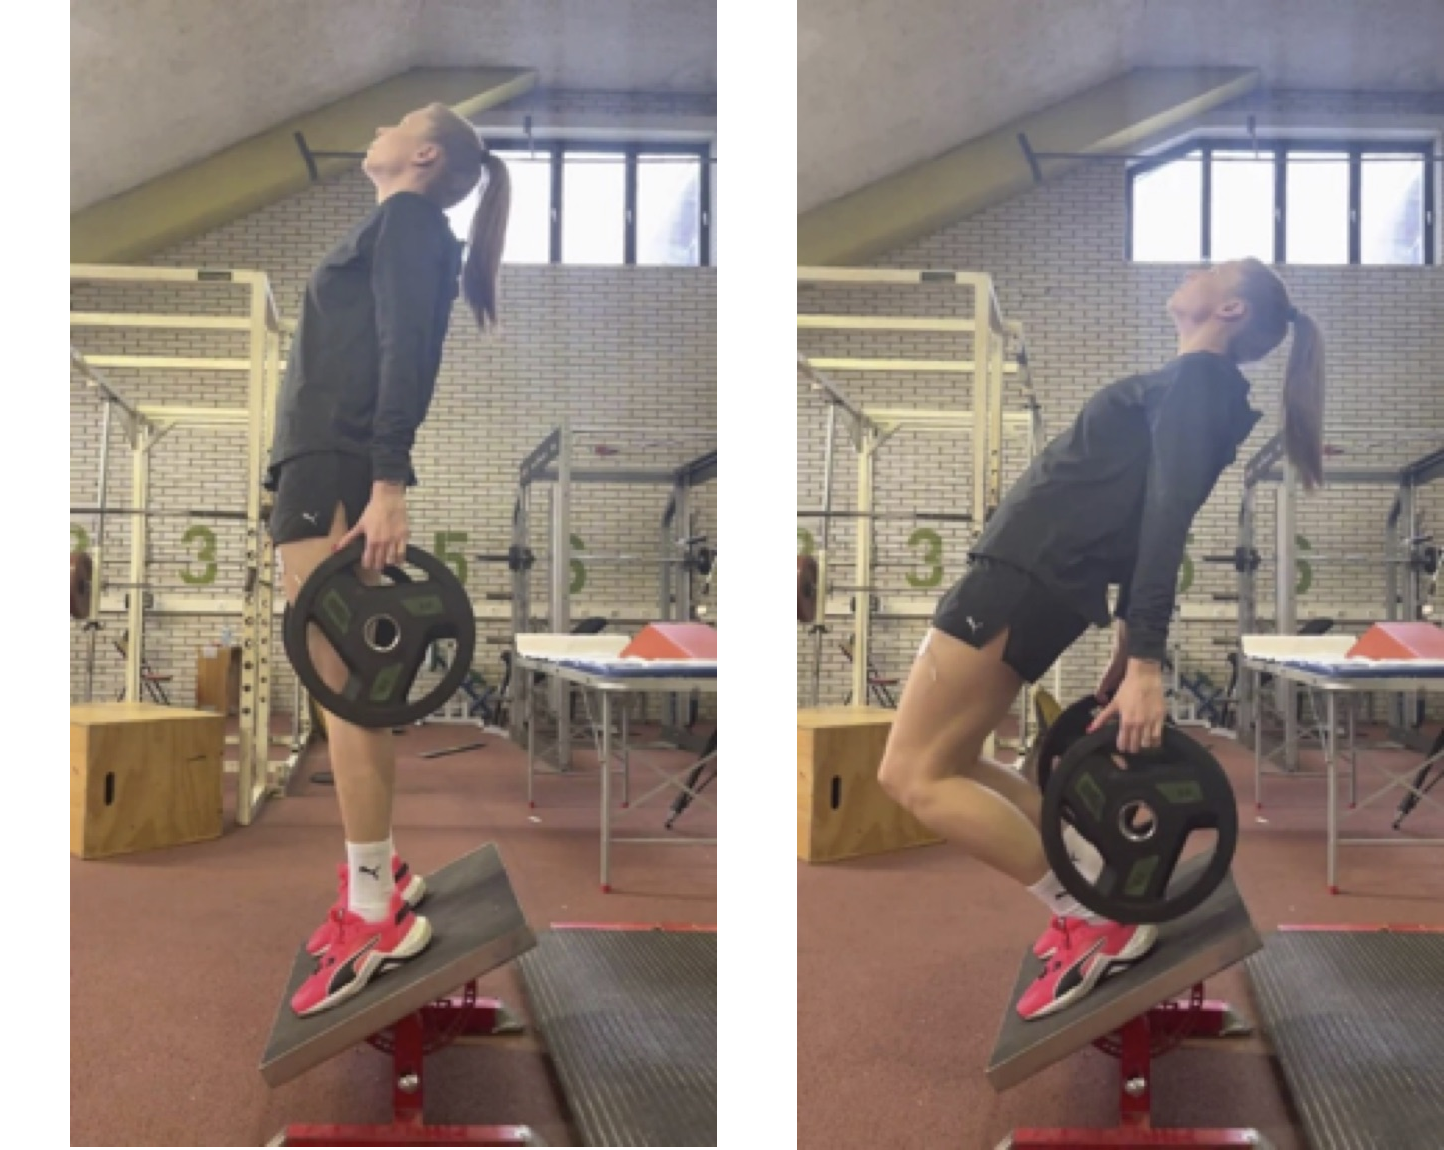
\includegraphics[width=0.65\textwidth]{word/isq.png}
    \caption{The incline squat used as a conditioning exercise.}
    \label{fig:isq}
\end{figure}

\subsubsection{Measurement Protocol}
The study used the following conditioning exercise and TMG measurement protocol:
\begin{enumerate}

    \item pre-conditioning (baseline) TMG measurement(s), followed within \SI{15}{\second} by...

    \item eight repetitions of ISQ, followed within \SI{12}{\second} by...

    \item post-conditioning TMG measurement(s), followed by...

    \item a rest period of \SI{150}{\second}.

\end{enumerate}
This four-step procedure is shown in Figure~\ref{fig:protocol} and was repeated eight times by each subject.
Two variations were used:
\begin{itemize}

    \item For subjects 1-16, eight pre-ISQ and eight post-ISQ TMG measurements were taken in rapid succession (less than \SI{1}{\second} between successive measurements) in each of the eight measurement sets, for a total of 64 pre-ISQ and 64 post-ISQ TMG measurements per subject.

    \item For subjects 17-54, one pre-ISQ and one post-ISQ TMG measurement was taken in each of the eight measurement sets, for a total of 8 pre-ISQ and 8 post-ISQ TMG measurements.

\end{itemize}

\begin{table}[htb!]
    \centering
    \caption{The number of TMG measurements taken per set depending on the subject.}
    \vspace{1ex}
    \begin{tabular}{|c|c|c|c|}
        \hline {\rule{0pt}{2.0ex}} \hspace{-7pt}
        Subjects & Pre-ISQ per set & Post-ISQ per set \\
        \hline {\rule{0pt}{2.0ex}} \hspace{-7pt}
        1-16 & 8 & 8 \\
        17-54 & 1 & 1 \\
        \hline
    \end{tabular}
    \label{tab:measurements}
\end{table}

\begin{figure}
	\centering
    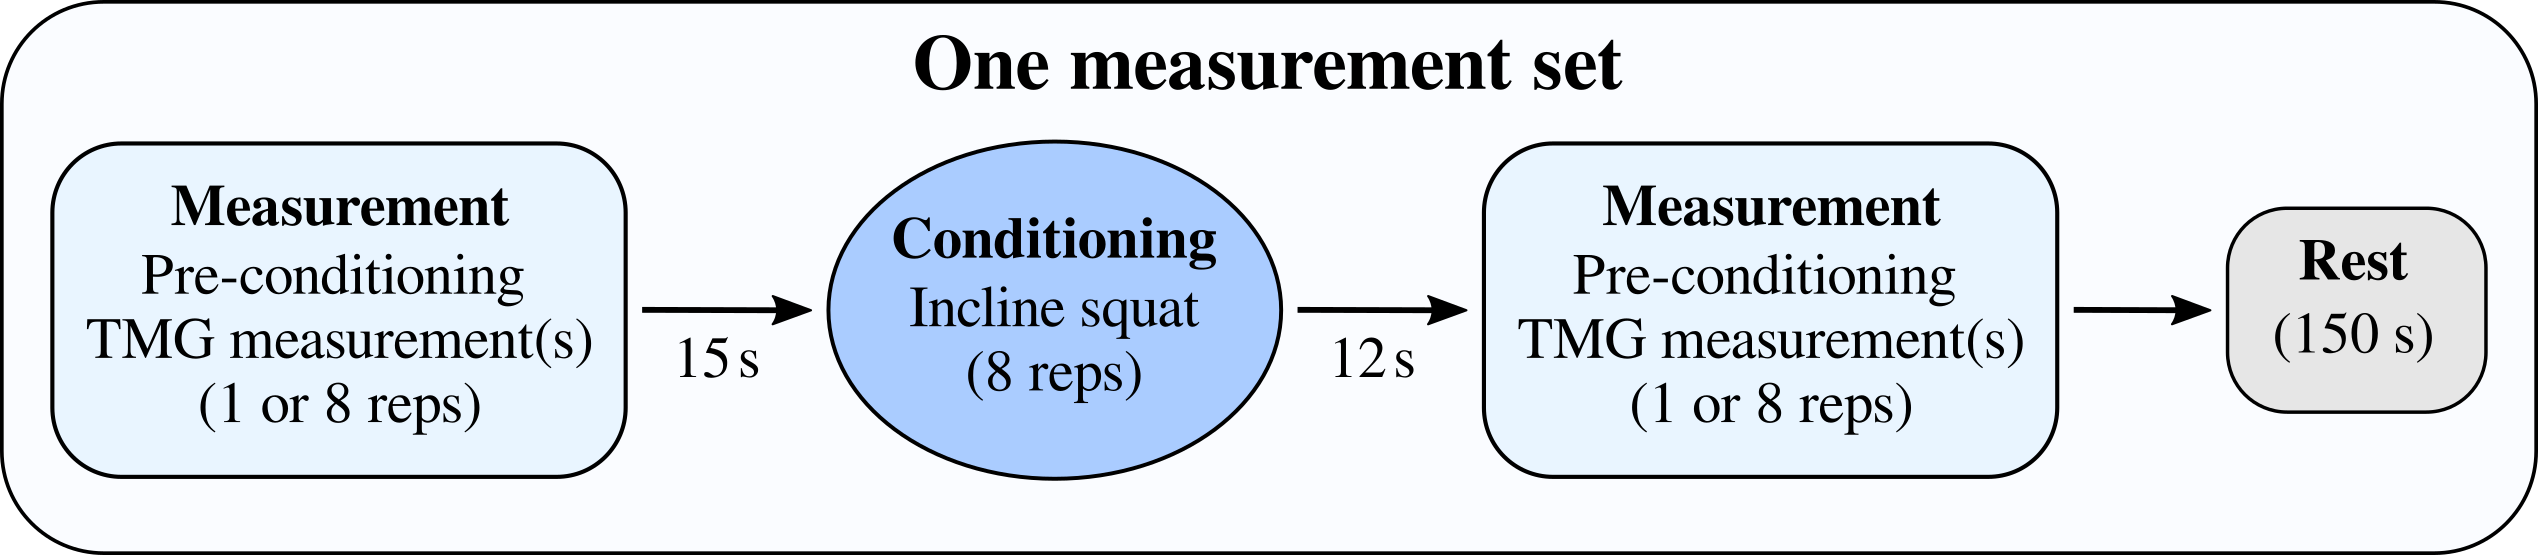
\includegraphics[width=\textwidth]{protocol-set.png}
    \caption{One set of the conditioning exercise and measurement protocol used in the study.
    This measurement set was repeated eight times over the course of the study.
    Eight pre-ISQ and eight post-ISQ TMG measurements were taken per set for subjects 1-16, while one pre-ISQ and one post-ISQ TMG measurement was taken per set for subjects 17-54.}
    \label{fig:protocol}
\end{figure}

\subsubsection{Estimated Load on the Quadriceps Muscle}
An inverse dynamics analysis of a three-segment planar human body model, assuming a quasi-static condition (see Appendix 1) [10][7][8], was used to estimate the load on the quadriceps muscles (especially the RF, which is loaded at the full amplitude of knee movement) during the ISQ.
The model's body segment properties were estimated using anthropometric data and the subject’s body height and body mass as input parameters [9].
% TODO: clarify with the anthropometric data is. Is this the distance from knee to foot?
The subjects' motion in the sagittal plane was recorded on video, and one exercise repetition was selected for estimating the inter-segmental angles (Figure 4).
The peak value of the net knee joint moment was estimated at the lowest body position in the ISQ,
and normalized to the volunteer’s body mass to reduce the effect of inter-subject variance [5][6].
The normalized peak values of the knee joint moment were used to compare the loading of the knee extensor muscles during the ISQ between the volunteers.

\subsection{Analysis of Muscle Contractile Response}

\subsubsection{Software}
Data analysis and standard statistical tests were performed in the Python 3 programming language (\url{https://www.python.org/}) using the Numpy and SciPy libraries (\url{https://numpy.org/}, \url{https://scipy.org/});
and with SPSS Statistics 20 (SPSS Inc., Chicago, IL, USA) and Microsoft Excel.
Statistical parametric mapping analysis was performed in Python 3 using the SPM1d library [34][35] (\url{https://www.spm1d.org}).

\subsubsection{Discrete Twitch Contraction Parameters} \label{sss:discrete_twitch_params}
The RF's contractile response was measured with TMG.
The TMG signal corresponds physically to muscle belly displacement with respect to time over the course of the muscle twitch.
The signal is sampled for \SI{1}{\second} at a sample rate of \SI{1}{\kilo \hertz}, for a total of 1000 data points.
A typical TMG signal and its time derivative are show in in Figure~\ref{fig:tmg_example}.
The following five discrete twitch contraction parameters were computed from every measured TMG signal.
\begin{enumerate}

    \item \Dm: maximum displacement of the muscle belly during contraction;

    \item \Td (delay time): time taken for muscle belly displacement to reach 10 percent of its maximum value;

    \item \Tc (contraction time): time taken for muscle belly displacement to change from 10 to 90 percent of its maximum value (analogous to the rise time parameter commonly used in electronics);

    \item \RDDMax (maximum rate of displacement development): the maximum rate of change of muscle belly displacement with respect to time, i.e. the maximum value of the TMG signal's time derivative;

    \item \RDDMaxTime: the time at which the TMG signal's time derivative attains its maximum value, i.e. the time at which \RDDMax occurs.

\end{enumerate}
Each of these parameters is marked in Figure~\ref{fig:tmg_example}.
To estimate post-activation potentiation, the five above-described twitch contraction parameters were computed for every TMG measurement for all subjects.
The pairwise differences in pre- and post-conditioning parameter values then served as indicators of potentiation.

\subsubsection{Statistical testing of discrete contraction parameters} \label{sss:discrete_twitch_param_stats}
One way to identify post-activation potentiation is simply to compare pre- and post-conditioning parameter values with the naked eye.
Appreciably larger values of \Dm (indicating larger twitch amplitude) and \RDDMax (indicating greater rate of force development), and appreciably smaller values of \Td, \Tc, and \RDDMaxTime (indicating a faster muscle response) in the post-conditioning response relative to the pre-conditioning response indicate post-activation twitch potentiation.

A more refined approach would use statistical hypothesis testing, and we adopt this method here.
For each of the five twitch contraction parameters, we assume the null hypothesis that pre- and post-conditioning parameter values were drawn from populations with the same mean
(interpreted more loosely, that any difference in pre- and post-conditioning values is due to chance alone and there is no meaningful difference in pre- and post-conditioning contraction properties)
and then test this hypothesis with a paired Student's $ t $-test.

Statistical testing imposes an important challenge: any binary hypothesis test must act on a large-enough sample size to have meaningful statistical power (i.e. probability of correctly rejecting the null hypothesis).
In the context of this study, this means any Student's $ t $-test comparing pre- and post-ISQ parameter values must act on a sample of \textit{many} pre- and post-ISQ pairs (while comparing only one pre-ISQ and one post-ISQ value would be statistically meaningless).
There is no exact answer on what sample size is ``large enough''; we use at least eight (pre-ISQ, post-ISQ) pairs in this study, while five pairs might serve as a tentative lower bound.
Assembling these pairs in a physically meaningful way can pose a challenge;
we considered the following three variations for each of the five twitch contraction parameters mentioned in Section~\ref{sss:discrete_twitch_params}:
\begin{enumerate}

    \item For subjects 1-16 (for whom 8 pre-ISQ and 8 post-ISQ TMG measurements were taken in each measurement set, see Table~\ref{tab:measurements}), we compare all 8 pre-ISQ parameter values from a given measurement set against all 8 post-ISQ parameter values from the same set.
    This comparison tests for potentiation after a single conditioning exercise set in a given subject.

    \item For subjects 17-54 (for whom 1 pre-ISQ and 1 post-ISQ TMG measurement was taken per measurement set, see Table~\ref{tab:measurements}), we compare the 8 pre-ISQ parameter values (one from each of the 8 measurement sets) to the corresponding post-ISQ parameter values.
    This comparison captures a single subject's muscle response over the entire 8-set measurement protocol, but cannot determine post-activation potentiation after a single exercise.

    \item For all subjects and for each measurement set we compare the 54 pre-ISQ parameter values to the 54 post-ISQ parameter values (using the first of eight measurements per set for subjects 1-16 and the only measurement per set for subjects 17-54).
    This comparison tests for a potentiation-like trend over all subjects as a whole, but is not useful for testing for potentiation in any given subject.

\end{enumerate}
Results appear in \TODO{reference}.

\begin{figure}
	\centering
    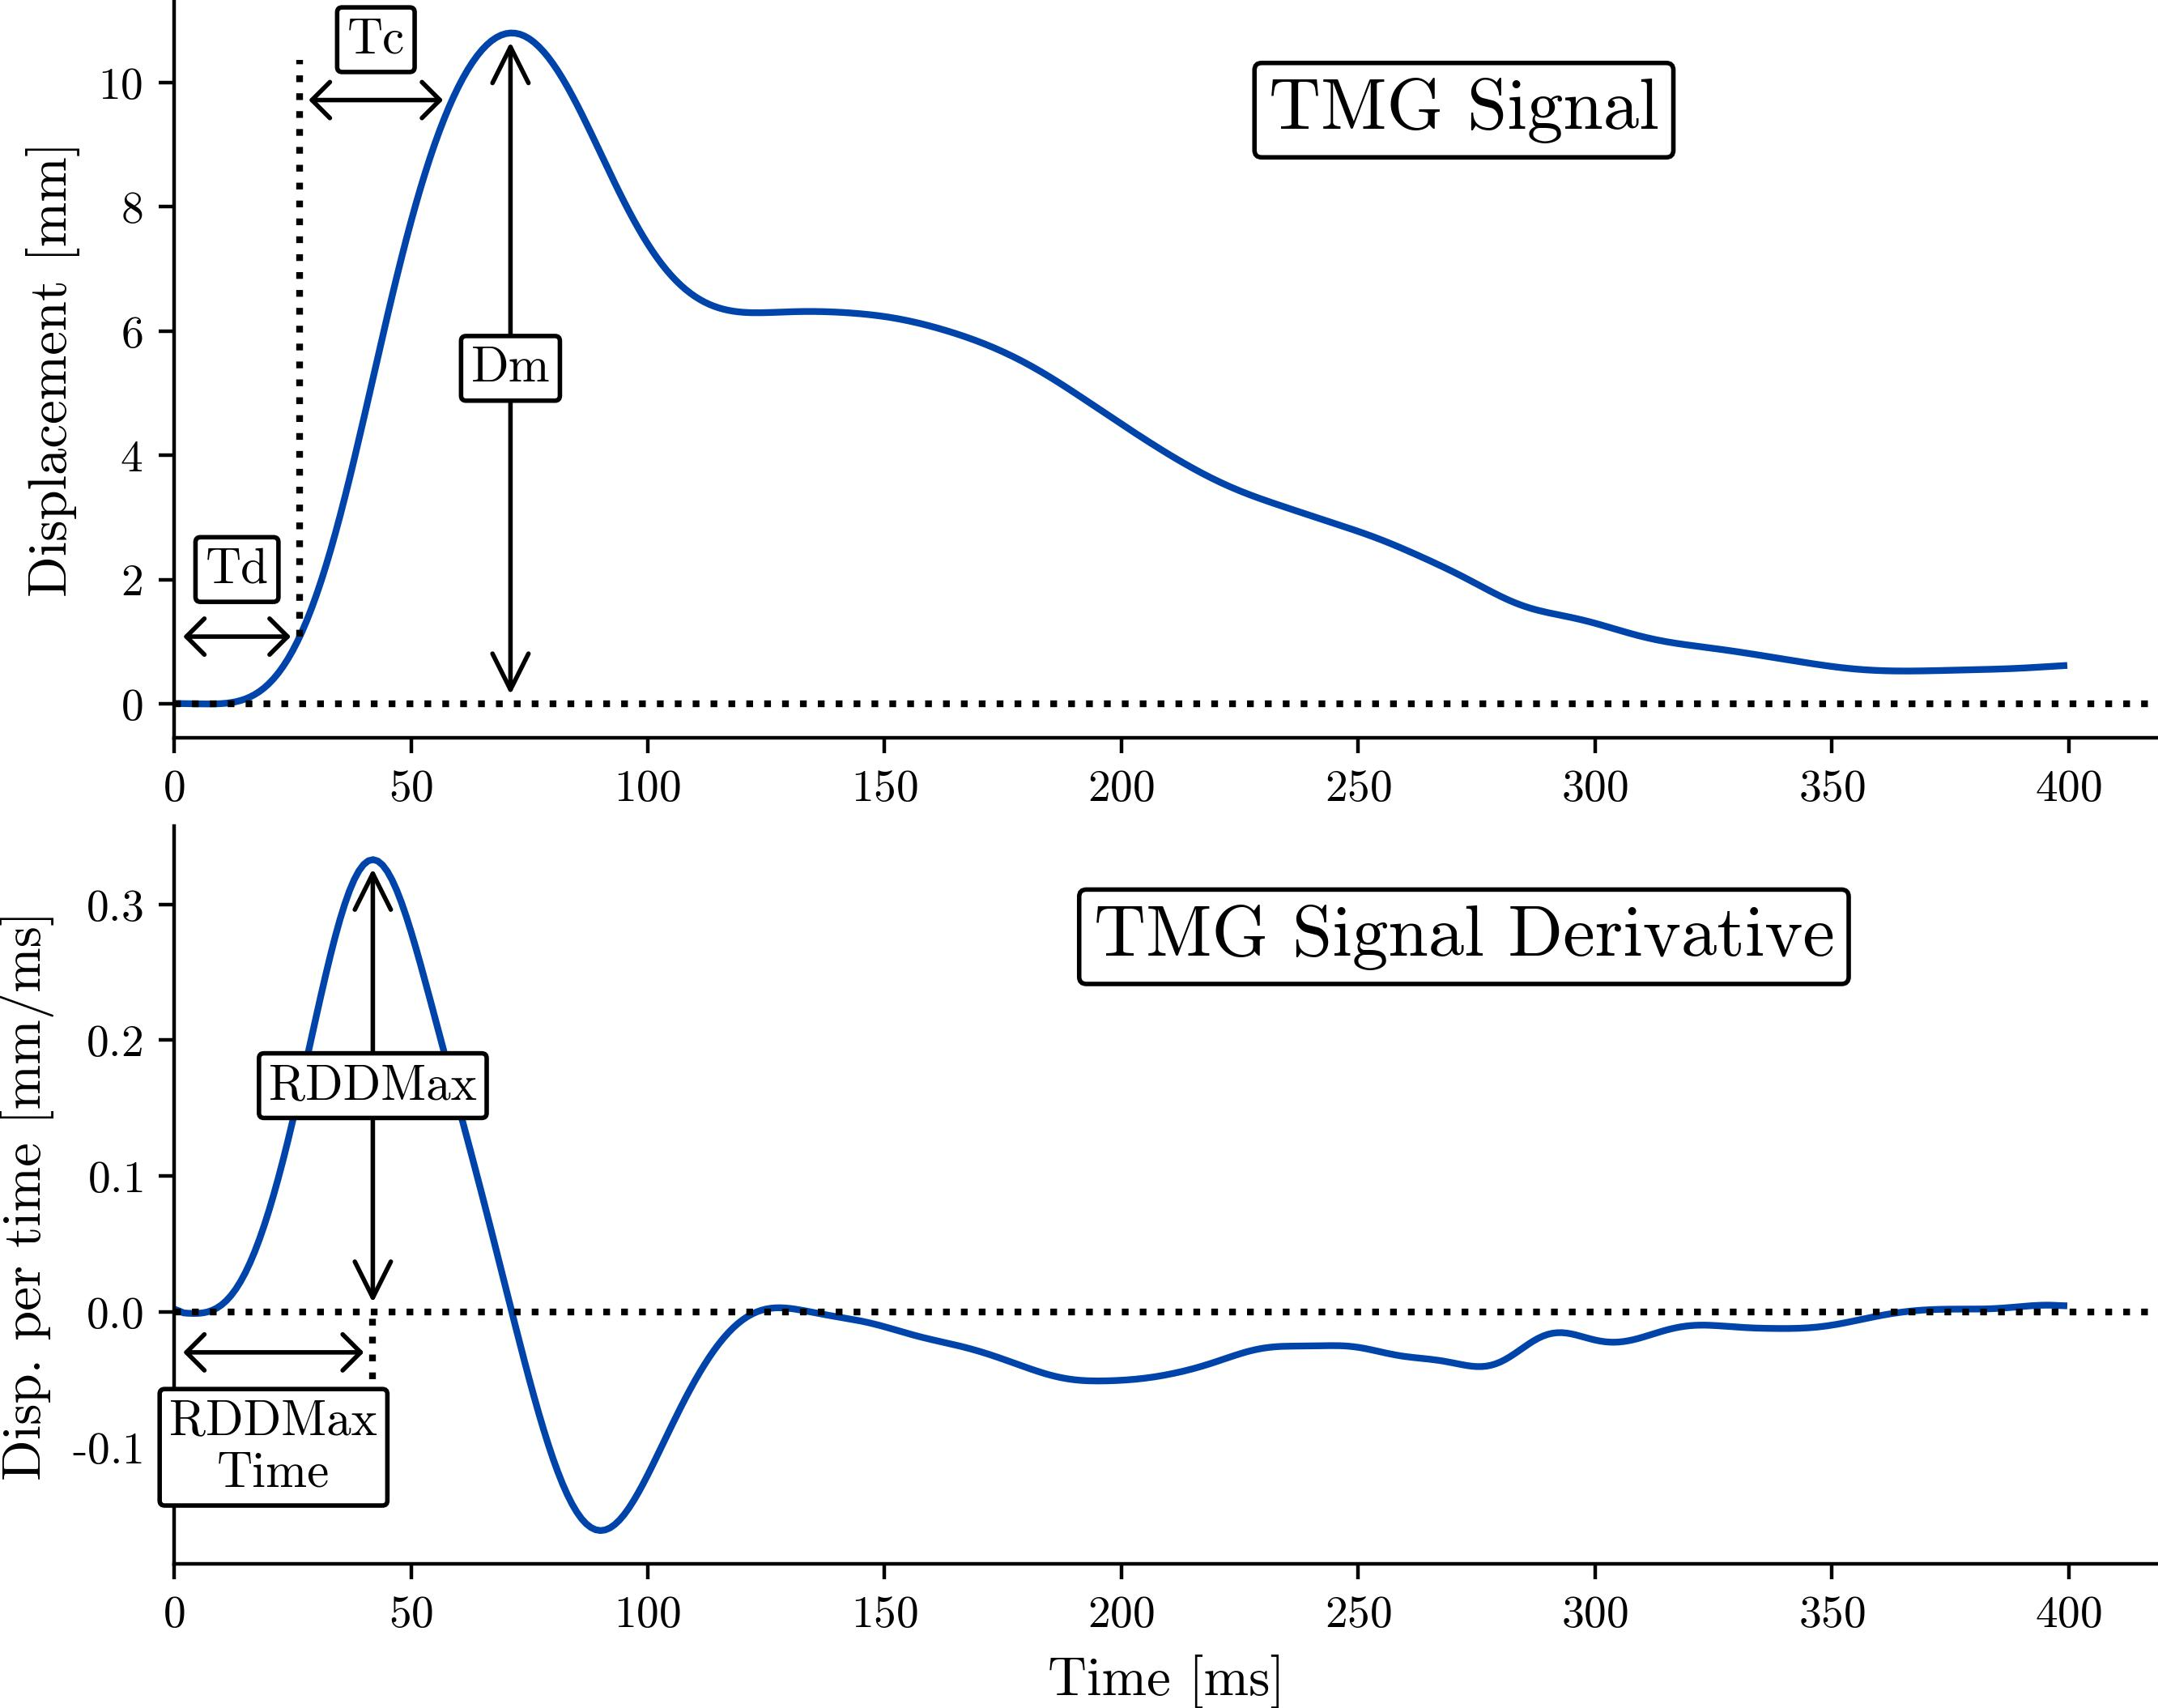
\includegraphics[width=\textwidth]{tmg-example.jpg}
    \caption{A representative TMG signal (top) and its derivative with respect to time (bottom), together with the discrete twitch contraction parameters used to summarize these signals.}
    \label{fig:tmg_example}
\end{figure}

\subsubsection{SPM Analysis}
Broadly speaking, classical statistical tests on zero-dimensional datasets quantify the probability that randomly-distributed scalar data would produce a test statistic exceeding a critical threshold value.
SPM-based statistical testing is a conceptually identical generalization to datasets consisting of continuous, and in our case one-dimensional,%
\footnote{In this study the signals are one-dimensional TMG signals encoding muscle belly displacement with respect to time, but SPM generalizes straightforwardly to arbitrary-dimensional random fields.}
\textit{signals}.
SPM testing quantifies the probability that smooth, 1D random fields would produce a test statistic continuum whose maximum exceeds a threshold test statistic value.

The study used one-dimensional paired SPM $ t $-tests to evaluate the effect of the ISQ conditioning exercise on the rectus femoris's twitch contraction properties in the time domain.
Pre-conditioning TMG signals were compared against post-conditioning TMG signals and statistically significant differences between the two were interpreted as indicating a potentiated post-conditioning response.
The first \SI{100}{\milli \second} of the RF twitch contraction response was used as the region of interest for SPM analysis, since this region entirely captures the muscle's contraction phase.

SPM testing of TMG signals follows a procedure analogous to the classical Student's $ t $-tests applied to the scalar twitch contraction parameters in Section~\ref{sss:discrete_twitch_param_stats}, only with the scalar parameters and associated scalar $ t $-statistic generalized to one-dimensional signals.
The analysis goes as follows.
\begin{enumerate}

    \item We first assume the null hypothesis that differences in a collection of pre- and post-conditioning TMG signals are due to chance alone.
    More formally, letting $ \mu_{\mathrm{pre}}(t) $ and $ \mu_{\mathrm{post}}(t) $ denote the mean pre- and post-conditioning TMG amplitudes at time $ t $, respectively, the null hypothesis is
    \begin{equation*}
        \mu_{\text{pre}}(t) - \mu_{\text{post}} (t) = 0 \text{ for all } t,
    \end{equation*}
    while the alternate hypothesis is $ \mu_{\text{post}}(t) > \mu_{\text{pre}}(t) $, i.e. a larger mean twitch amplitude in post-conditioning TMG signals.

    \item We then use the set of pre- and post-conditioning signals with the \texttt{stats.ttest\_paired} function provided by the SPM1d library to construct a one-dimensional \textit{statistical parameteric map}.
    This map, also called the \textit{SPM $ t $-continuum}, serves to quantify the difference in the pre- and post-conditioning TMG signals at each point in time.
    (Much like the classical, scalar $ t $-statistic associated with scalar twitch contraction parameters quantifies the difference between the pre- and post-conditioning parameter values.)

    \item Finally, we perform a one-tailed\footnote{We make a one-tailed (and not two-tailed) inference under the a priori hypothesis that post-conditioning TMG signals will be larger-amplitude than pre-conditioning signals.} SPM inference on the SPM $ t $-continuum at the significance level $ \alpha = 0.01 $ using the \texttt{inference} function provided by the SPM1d library's \texttt{SPM\_T} class.
 
\end{enumerate}
The final inference step produces a threshold $ t $-statistic value $ t^{*} $, which is the threshold at which the maximum value of an SPM $ t $-continuum generated by smooth, Gaussian random continuua (as opposed to, say, TMG signals) would exceed $ t^{*} $ with probability $ \alpha $.
From the perspective of classical hypothesis testing, we reject the null hypothesis at the significance level $ \alpha $ if the SPM $ t $-continuum generated from the pre- and post-conditioning TMG signals exceeds $ t^{*} $.

The final inference step also produces a probability value $ p $ associated with each supra-threshold region of the SPM $ t $-continuum.
This $ p $ value represents the probability that smooth, Gaussian random continuua would produce a supra-threshold region as wide or wider (relative to the width of the entire SPM $ t $-continuum) than the supra-threshold region observed in the SPM $ t $-continuum computed from the measured TMG signals.
For orientation, a representative set of pre- and post-conditioning TMG signals, the SPM $ t $-continuum computed from them, and the associated threshold value $ t^{*} $ appear in Figure~\ref{fig:spm_example}.

\begin{figure}
	\centering
    \includegraphics[width=\textwidth]{spm-example.jpg}
    \caption{A representative set of pre- and post-conditioning TMG signals (left) and the resulting SPM $ t $-continuum and threshold value $ t^{*} $.
    Note the larger amplitude and shorter time to peak contraction in the post-ISQ signal.}
    \label{fig:spm_example}
\end{figure}

We performed SPM testing with the same three configurations described in Section~\ref{sss:discrete_twitch_param_stats} for classical hypothesis testing of discrete twitch contraction parameters.
\begin{enumerate}

    \item For subjects 1-16, we compare all 8 pre-ISQ TMG signals from a given measurement set against all 8 post-ISQ TMG signals from the same set.

    \item For subjects 17-54, we compare one pre-ISQ TMG signals from each of the eight measurement sets (for a total of eight pre-ISQ signals) to the corresponding eight post-ISQ TMG signals.

    \item For all subjects and for each measurement set, we compare one pre-ISQ TMG signal and one post-ISQ TMG signal from each subject (using the first of the eight measurements per set for subjects 1-16 and the only measurement per set for subjects 17-54), for a total of 54 (pre-ISQ, post-ISQ) TMG signal pairs.

\end{enumerate}
Results appear in \TODO{reference}.

\subsubsection{Summary parameters of SPM}
To complement the SPM $ t $-continuum generated from each SPM paired $ t $-test (see Figure~\ref{fig:spm_example} for an example), we collected and/or calculated the following discrete parameters to make the SPM result easier to compare at a glance.
\begin{itemize}

    \item \SPMStart: time at which the supra-threshold cluster begins
    \item \SPMEnd: time at which the supra-threshold cluster ends
    \item \SPMCentroidTime: the time of the supra-threshold cluster's centroid in the time, $ t $-continuum plane.
    \item \SPMCentroidT: the $ t $-continuum value of the supra-threshold cluster's centroid in the time, $ t $-continuum plane.
    \item \SPMMax: the maximum value of the SPM $ t $-continuum.
    \item \SPMArea: The area of the supra-threshold cluster.

\end{itemize}
All parameters besides \SPMArea are directly provided by the SPM1d library, while \SPMArea was computed using the trapezoid method for numerical integration using the SPM $ t $-continuum and threshold value $ t^{*} $.

\section{Results}
\subsection{Discrete twitch contraction parameters}

Show mean and SD of TMG graph.
Show table of parameter values.

\subsubsection{Sample: in a set for a given subject}

\subsubsection{Sample: across sets for a given subject}

\subsubsection{Across subjects for a given set}
In all four measurement sets, the difference in the volunteers' pre-ISQ and post-ISQ twitch contraction parameters 
(\Td, \Tc, \Dm, \RDDMax, and \RDDMaxTime)
was statistically significant, with a $ p $ value $ p < 0.0001 $ when tested with a dependent Student's $ t $-test for paired samples at a significance level $ \alpha = 0.05 $.
The study used two related schemes to compare pre- and post-ISQ twitch contraction parameters:
\begin{enumerate}

    \item In the first method, pre- and post-ISQ twitch contraction parameters are compared set by set;
    the parameter values appear in Table~\ref{tab:tmg_params}.

    \item In the second method, post-ISQ twitch parameters in each set are compared to the pre-ISQ parameters in the \textit{first} set;
    the parameter values appear in Table~\ref{tab:tmg_params_staggered}.
    % TODO: reasoning why this method is used.

\end{enumerate}

\begin{table}[htb!]
    \centering
    \caption{Set-by-set comparison of pre- and post-ISQ twitch contraction parameter values averaged across all subjects---note the consistent, potentiation-like increase in muscle amplitude and decrease in contraction time following ISQ.
    The difference between pre- and post-ISQ values for all parameters was statistically with a $ p $ value $ p < 0.0001 $ when tested with a Student's $ t $-test for paired samples at a significance level $ \alpha = 0.05 $.
    Parameters were introduced in Materials and Methods; for review:
    \Dm is maximum displacement of TMG sensor from muscle belly;
    \Td is time from start of TMG signal to 10\% of its maximum value \Dm;
    \Tc is time from 10\% of \Dm to 90\% of \Dm;
    \RDDMax is maximum value of the TMG signal's time derivative,
    \RDDMaxTime is time at which \RDDMax occurs.
    }
    \vspace{1ex}

    \renewcommand{\arraystretch}{1.2}
    \begin{tabular}{|c|l|c|c|c|c|}
    \hline {\rule{0pt}{2.0ex}} \hspace{-7pt}
    Parameter & & Set 1 & Set 2 & Set 3 & Set 4\\
    \hline
    \hline {\rule{0pt}{2.0ex}} \hspace{-7pt}
    
    % Dm
    \multirow{3}{*}{\textbf{Dm}} & Mean PR $ [\si{\milli \meter}] $ & $8.71$ & $9.21$ & $9.07$ & $9.13$\\
     & Mean PO $ [\si{\milli \meter}] $ & $10.06$ & $10.10$ & $10.15$ & $9.95$\\
     & Percent difference & $+15.42$\% & $+9.70$\% & $+11.83$\% & $+8.96$\%\\
    \hline {\rule{0pt}{2.0ex}} \hspace{-7pt}
    
    % Td
    \multirow{3}{*}{\textbf{Td}} & Mean PR $ [\si{\milli \second}] $ & $25.28$ & $24.97$ & $24.01$ & $24.39$\\
     & Mean PO $ [\si{\milli \second}] $ & $22.46$ & $22.15$ & $21.94$ & $21.85$\\
     & Percent difference & $-11.17$\% & $-11.28$\% & $-8.64$\% & $-10.41$\%\\
    \hline {\rule{0pt}{2.0ex}} \hspace{-7pt}
    
    % Tc
    \multirow{3}{*}{\textbf{Tc}} & Mean PR $ [\si{\milli \second}] $ & $31.38$ & $30.59$ & $29.36$ & $28.94$\\
     & Mean PO $ [\si{\milli \second}] $ & $26.17$ & $25.24$ & $24.92$ & $24.56$\\
     & Percent difference & $-16.61$\% & $-17.51$\% & $-15.12$\% & $-15.12$\%\\
    \hline {\rule{0pt}{2.0ex}} \hspace{-7pt}
    
    % RDD max
    \multirow{3}{*}{\textbf{$ \text{RDD}_{\text{max}} $}} & Mean PR $ [\si{\milli \meter \per \milli \second}] $ & $0.27$ & $0.29$ & $0.30$ & $0.31$\\
     & Mean PO $ [\si{\milli \meter \per \milli \second}] $ & $0.37$ & $0.39$ & $0.40$ & $0.39$\\
     & Percent difference & $+39.52$\% & $+35.10$\% & $+31.25$\% & $+27.46$\%\\
    \hline {\rule{0pt}{2.0ex}} \hspace{-7pt}
    
    % RDD max time
    \multirow{3}{*}{\textbf{$ \text{TRDD}_{\text{max}} $}} & Mean PR $ [\si{\milli \second}] $ & $41.03$ & $39.66$ & $38.72$ & $38.55$\\
     & Mean PO $ [\si{\milli \second}] $ & $36.56$ & $35.28$ & $35.15$ & $35.30$\\
     & Percent difference & $-10.90$\% & $-11.04$\% & $-9.24$\% & $-8.43$\%\\
    \hline
\end{tabular}

    \label{tab:tmg_params}
\end{table}

\begin{table}[htb!]
    \centering
    \caption{Post-ISQ twitch contraction parameter values from sets 1, 2, 3, and 4 compared to the pre-ISQ values from set 1,
    so mean pre-ISQ values are shown only for set 1.
    All parameters have the same meanings as in Table~\ref{tab:tmg_params}.
    As in Table~\ref{tab:tmg_params}, note the consistent, potentiation-like increase in muscle amplitude and decrease in contraction time.
    }
    \vspace{1ex}

    \renewcommand{\arraystretch}{1.2}
    \begin{tabular}{|c|l|c|c|c|c|}
    \hline {\rule{0pt}{2.0ex}} \hspace{-7pt}
    Parameter & & Set 1 & Set 2 & Set 3 & Set 4\\
    \hline
    \hline {\rule{0pt}{2.0ex}} \hspace{-7pt}
    
    % Dm
    \multirow{3}{*}{\textbf{Dm}} & Mean PR $ [\si{\milli \meter}] $ & $8.71$ & - & - & -\\
     & Mean PO $ [\si{\milli \meter}] $ & $10.06$ & $10.10$ & $10.15$ & $9.95$\\
     & Percent difference & $+15.42$\% & $+15.95$\% & $+16.44$\% & $+14.17$\%\\
    \hline {\rule{0pt}{2.0ex}} \hspace{-7pt}
    
    % Td
    \multirow{3}{*}{\textbf{Td}} & Mean PR $ [\si{\milli \second}] $ & $25.28$ & - & - & -\\
     & Mean PO $ [\si{\milli \second}] $ & $22.46$ & $22.15$ & $21.94$ & $21.85$\\
     & Percent difference & $-11.17$\% & $-12.38$\% & $-13.22$\% & $-13.58$\%\\
    \hline {\rule{0pt}{2.0ex}} \hspace{-7pt}
    
    % Tc
    \multirow{3}{*}{\textbf{Tc}} & Mean PR $ [\si{\milli \second}] $ & $31.38$ & - & - & -\\
     & Mean PO $ [\si{\milli \second}] $ & $26.17$ & $25.24$ & $24.92$ & $24.56$\\
     & Percent difference & $-16.61$\% & $-19.59$\% & $-20.60$\% & $-21.73$\%\\
    \hline {\rule{0pt}{2.0ex}} \hspace{-7pt}
    
    % RDD max
    \multirow{3}{*}{\textbf{$ \text{RDD}_{\text{max}} $}} & Mean PR $ [\si{\milli \meter \per \milli \second}] $ & $0.27$ & - & - & -\\
     & Mean PO $ [\si{\milli \meter \per \milli \second}] $ & $0.37$ & $0.39$ & $0.40$ & $0.39$\\
     & Percent difference & $+39.52$\% & $+46.89$\% & $+48.16$\% & $+45.62$\%\\
    \hline {\rule{0pt}{2.0ex}} \hspace{-7pt}
    
    % RDD max time
    \multirow{3}{*}{\textbf{$ \text{TRDD}_{\text{max}} $}} & Mean PR $ [\si{\milli \second}] $ & $41.03$ & - & - & -\\
     & Mean PO $ [\si{\milli \second}] $ & $36.56$ & $35.28$ & $35.15$ & $35.30$\\
     & Percent difference & $-10.90$\% & $-14.02$\% & $-14.35$\% & $-13.97$\%\\
    \hline
\end{tabular}

    \label{tab:tmg_params_staggered}
\end{table}

SPM anaysis of TMG measurements using a two-sample SPM $ t $-test showed a statistically significant difference in pre-ISQ and post-ISQ muscle twitch in all four sets, in each case with a p-value $ p < 0.0001 $ at a significance level $ \alpha = 0.05 $.
The first \SI{100}{\milli \second} of the TMG signal were used as the region of interest for all SPM analyses, because this is the region in which both the maximal amplitude of twitch contraction and the phase of twitch amplitude decrease occur.
The results of each set's SPM $ t $-tests are plotted in Figure~\ref{fig:spm_plot}, while discrete parameters summarizing each set's SPM test appear in Table~\ref{tab:spm_params}.
% The value of the SPM $ t $-statistic significance threshold $ t^{*} $ remained approximately constant across all four measurement sets, ranging between $ t^{*} = 2.76 $ and $ t^{*} = 2.79 $.

\begin{figure}
	\centering
    \includegraphics[width=\textwidth]{spm-plot.jpg}
    \caption{For all four sets, a two-sample SPM $ t $-test comparing the first \SI{100}{\milli \second} of normalized pre- and post-ISQ TMG measurements across all subjects found a statistically significant difference between pre- and post-ISQ muscle twitch responses.
    The left column shows mean normalized pre-ISQ (black solid line) and post-ISQ (red solid line) TMG measurements, together with their standard deviation clouds, across all subjects for each measurement set.
    The right column shows the results of the SPM $ t $-test for each set;
    the dashed line denotes the threshold $ t^{*} $ at which each set's pre- and post-ISQ TMG signals differ significantly, while the maroon cloud emphasizes the region of significance.}
    \label{fig:spm_plot}
\end{figure}

\begin{table}[htb!]
    \centering
    \caption{
        Discrete parameters summarizing the results of the two-sample SPM $ t $-tests show in Figure~\ref{fig:spm_plot}.
        Parameters were introduced in Materials and Methods; for review:
        ``Start time'' is the time at which the SPM $ t $-statistic attains the significance threshold value $ t^{*} $;
        ``End time'' is the time at which the SPM $ t $-statistic falls below the significance threshold value $ t^{*} $;
        ``Centroid time'' and ``Centroid $ t $-value'' give the (time, $ t $) coordinate of the SPM significance region's centroid (the region shown in maroon in Figure~\ref{fig:spm_plot});
        ``SPM maximum'' is maximum value attained by the SPM $ t $-statistic;
        ``Area above threshold'' is area of the SPM significance region.
    }
    \vspace{1ex}

    \renewcommand{\arraystretch}{1.1}
    \begin{tabular}{|l|c|c|c|c|}
    \hline {\rule{0pt}{2.0ex}} \hspace{-7pt}
    SPM Parameters & Set 1 & Set 2 & Set 3 & Set 4\\
    \hline
    \hline {\rule{0pt}{2.0ex}} \hspace{-7pt}
    Start time $ [\si{\milli \second}] $ & 10.37 & 10.63 & 10.07 & 9.87\\[0.3ex]
    End time $ [\si{\milli \second}] $ & 57.82 & 57.67 & 56.11 & 56.84\\[0.3ex]
    Centroid time $ [\si{\milli \second}] $ & 33.32 & 34.14 & 32.17 & 32.56\\[0.3ex]
    Centroid $ t $-value & 6.78 & 8.08 & 6.90 & 7.06\\[0.3ex]
    SPM maximum & 7.77 & 9.49 & 8.28 & 8.12\\[0.3ex]
    Area above threshold & 195.1 & 259.5 & 198.5 & 209.9\\[0.3ex]
    \hline
\end{tabular}

    \label{tab:spm_params}
\end{table}

As an estimate of muscle load, the calculated mean value of peak knee torque during the ISQ was \SI{126.5 \pm 17.6}{\newton \meter}.

\section{Discussion}

\section*{Conflict of Interest Statement}
The authors declare that the research was conducted in the absence of any commercial or financial relationships that could be construed as a potential conflict of interest.

\section*{Author Contributions}
The Author Contributions statement must describe the contributions of individual authors referred to by their initials and, in doing so, all authors agree to be accountable for the content of the work.
Please see \href{https://www.frontiersin.org/about/policies-and-publication-ethics#AuthorshipAuthorResponsibilities}{here} for full authorship criteria.

\section*{Funding}
Details of all funding sources should be provided, including grant numbers if applicable.
Please ensure to add all necessary funding information, as after publication this is no longer possible.

\section*{Acknowledgments}
This is a short text to acknowledge the contributions of specific colleagues, institutions, or agencies that aided the efforts of the authors.

\section*{Supplemental Data}
 \href{http://home.frontiersin.org/about/author-guidelines#SupplementaryMaterial}{Supplementary Material} should be uploaded separately on submission, if there are Supplementary Figures, please include the caption in the same file as the figure. LaTeX Supplementary Material templates can be found in the Frontiers LaTeX folder.

\bibliographystyle{Frontiers-Harvard}
\bibliography{test}
%%% Please see the test.bib file for some examples of references

\end{document}
